\documentclass[paper=a4, fontsize=11pt]{scrartcl} % A4 paper and 11pt font size

\usepackage{placeins}
\usepackage{float}

\usepackage[T1]{fontenc} % Use 8-bit encoding that has 256 glyphs
\usepackage{fourier} % Use the Adobe Utopia font for the document - comment this line to return to the LaTeX default
\usepackage[english]{babel} % English language/hyphenation
\usepackage{amsmath,amsfonts,amsthm} % Math packages
\usepackage{mathtools}
\usepackage{graphicx}

\usepackage{lipsum} % Used for inserting dummy 'Lorem ipsum' text into the template
\usepackage{booktabs} % For \toprule, \midrule, \bottomrule in tables

\usepackage{sectsty} % Allows customizing section commands
\allsectionsfont{\centering \normalfont\scshape} % Make all sections centered, the default font and small caps

\usepackage{color} % or xcolor
\usepackage{soul}

\usepackage{fancyhdr} % Custom headers and footers
\pagestyle{fancyplain} % Makes all pages in the document conform to the custom headers and footers
\fancyhead{} % No page header - if you want one, create it in the same way as the footers below
\fancyfoot[L]{} % Empty left footer
\fancyfoot[C]{} % Empty center footer
\fancyfoot[R]{\thepage} % Page numbering for right footer
\renewcommand{\headrulewidth}{0pt} % Remove header underlines
\renewcommand{\footrulewidth}{0pt} % Remove footer underlines
\setlength{\headheight}{13.6pt} % Customize the height of the header

\numberwithin{equation}{section} % Number equations within sections (i.e. 1.1, 1.2, 2.1, 2.2 instead of 1, 2, 3, 4)
\numberwithin{figure}{section} % Number figures within sections (i.e. 1.1, 1.2, 2.1, 2.2 instead of 1, 2, 3, 4)
\numberwithin{table}{section} % Number tables within sections (i.e. 1.1, 1.2, 2.1, 2.2 instead of 1, 2, 3, 4)

\setlength\parindent{0pt} % Removes all indentation from paragraphs - comment this line for an assignment with lots of text

\newtheorem{definition}{Definition}
\newtheorem{theorem}{Theorem}

%----------------------------------------------------------------------------------------
%	TITLE SECTION
%----------------------------------------------------------------------------------------

\newcommand{\horrule}[1]{\rule{\linewidth}{#1}} % Create horizontal rule command with 1 argument of height

\title{	
\normalfont \normalsize 
\textsc{Princeton University, Applied Dynamical Systems} \\ [25pt] % Your university, school and/or department name(s)
\horrule{0.5pt} \\[0.4cm] % Thin top horizontal rule
\huge Oja-Type Plasticity and Neural Signal Reconstruction in Recurrent Networks  \\ % The assignment title
\horrule{2pt} \\[0.5cm] % Thick bottom horizontal rule
}

\author{David Hovey \& Aditya Biswas} % Your name

\date{\normalsize\today} % Today's date or a custom date

\begin{document}

\maketitle % Print the title

%----------------------------------------------------------------------------------------
%	PROBLEM 1
%----------------------------------------------------------------------------------------

\section{Introduction}
Do at end

\section{Motivation}
For Adi to do MENTION RESERVIOR COMPUTING

\section{Background}
\subsection{Fixed-Weight Recurrent Networks}

\subsection{Grossberg \(S\)-\(\Sigma\) Equivalence}

\subsection{Learning in Recurrent Neural Networks}

\subsection{Girko's Circular Law}
Fixed-weight recurrent networks are typically studied through deterministic methods such as fixed-point stability analysis. However, with Oja-type plasticity, we must study a higher-dimensional augmented system of weights and neural activity with  complex interactions. Probabilistic methods allow us to relax some of the dependence on exact trajectory-level analysis and instead study typical behavior across ensembles of networks. Motivated by the use of random weight initializations in reservoir computing,
we utilize Girko's circular law to analyze the evolution of the eigenvalues of our weight matrix. 

Let \(W^{(n)} = (W_{ij}) \in \mathbb{R}^{n \times n}\) be a random matrix whose entries are
independent and identically distributed (i.i.d.) real random variables satisfying
\[
\mathbb{E}[W_{ij}] = 0,
\qquad
\mathbb{E}[W_{ij}^2] = \frac{g^2}{n}
\]

Let \(\lambda_1,\dots,\lambda_n \in \mathbb{C}\) denote the eigenvalues of \(W^{(n)}\), and define the empirical spectral measure
\[
\mu_n
=
\frac{1}{n}\sum_{k=1}^n \delta_{\lambda_k}.
\]

Then Girko's circular law states that, as \(n \to \infty\),
\[
\mu_n \;\Rightarrow\; \mu_{\mathrm{circ}},
\]
where \(\Rightarrow\) denotes weak convergence of probability measures and
\[
d\mu_{\mathrm{circ}}(z)
=
\frac{1}{\pi g^2}\mathbf{1}_{\{|z|\le g\}}\, d^2 z
\]
is the uniform probability measure on the disk of radius \(g\) in \(\mathbb{C}\). 

For a sufficiently large system of $n$ neurons with weights sampled from $ \mathcal{N}(0, \frac{g^2}{n})$, Girko's Circular Law predicts that the eigenvalues of the neural weight matrix distribute uniformly on the disk
\[
D_g = \{ z \in \mathbb{C} \mid |z| \le g\}.
\]
\begin{figure}[H]
    \centering
    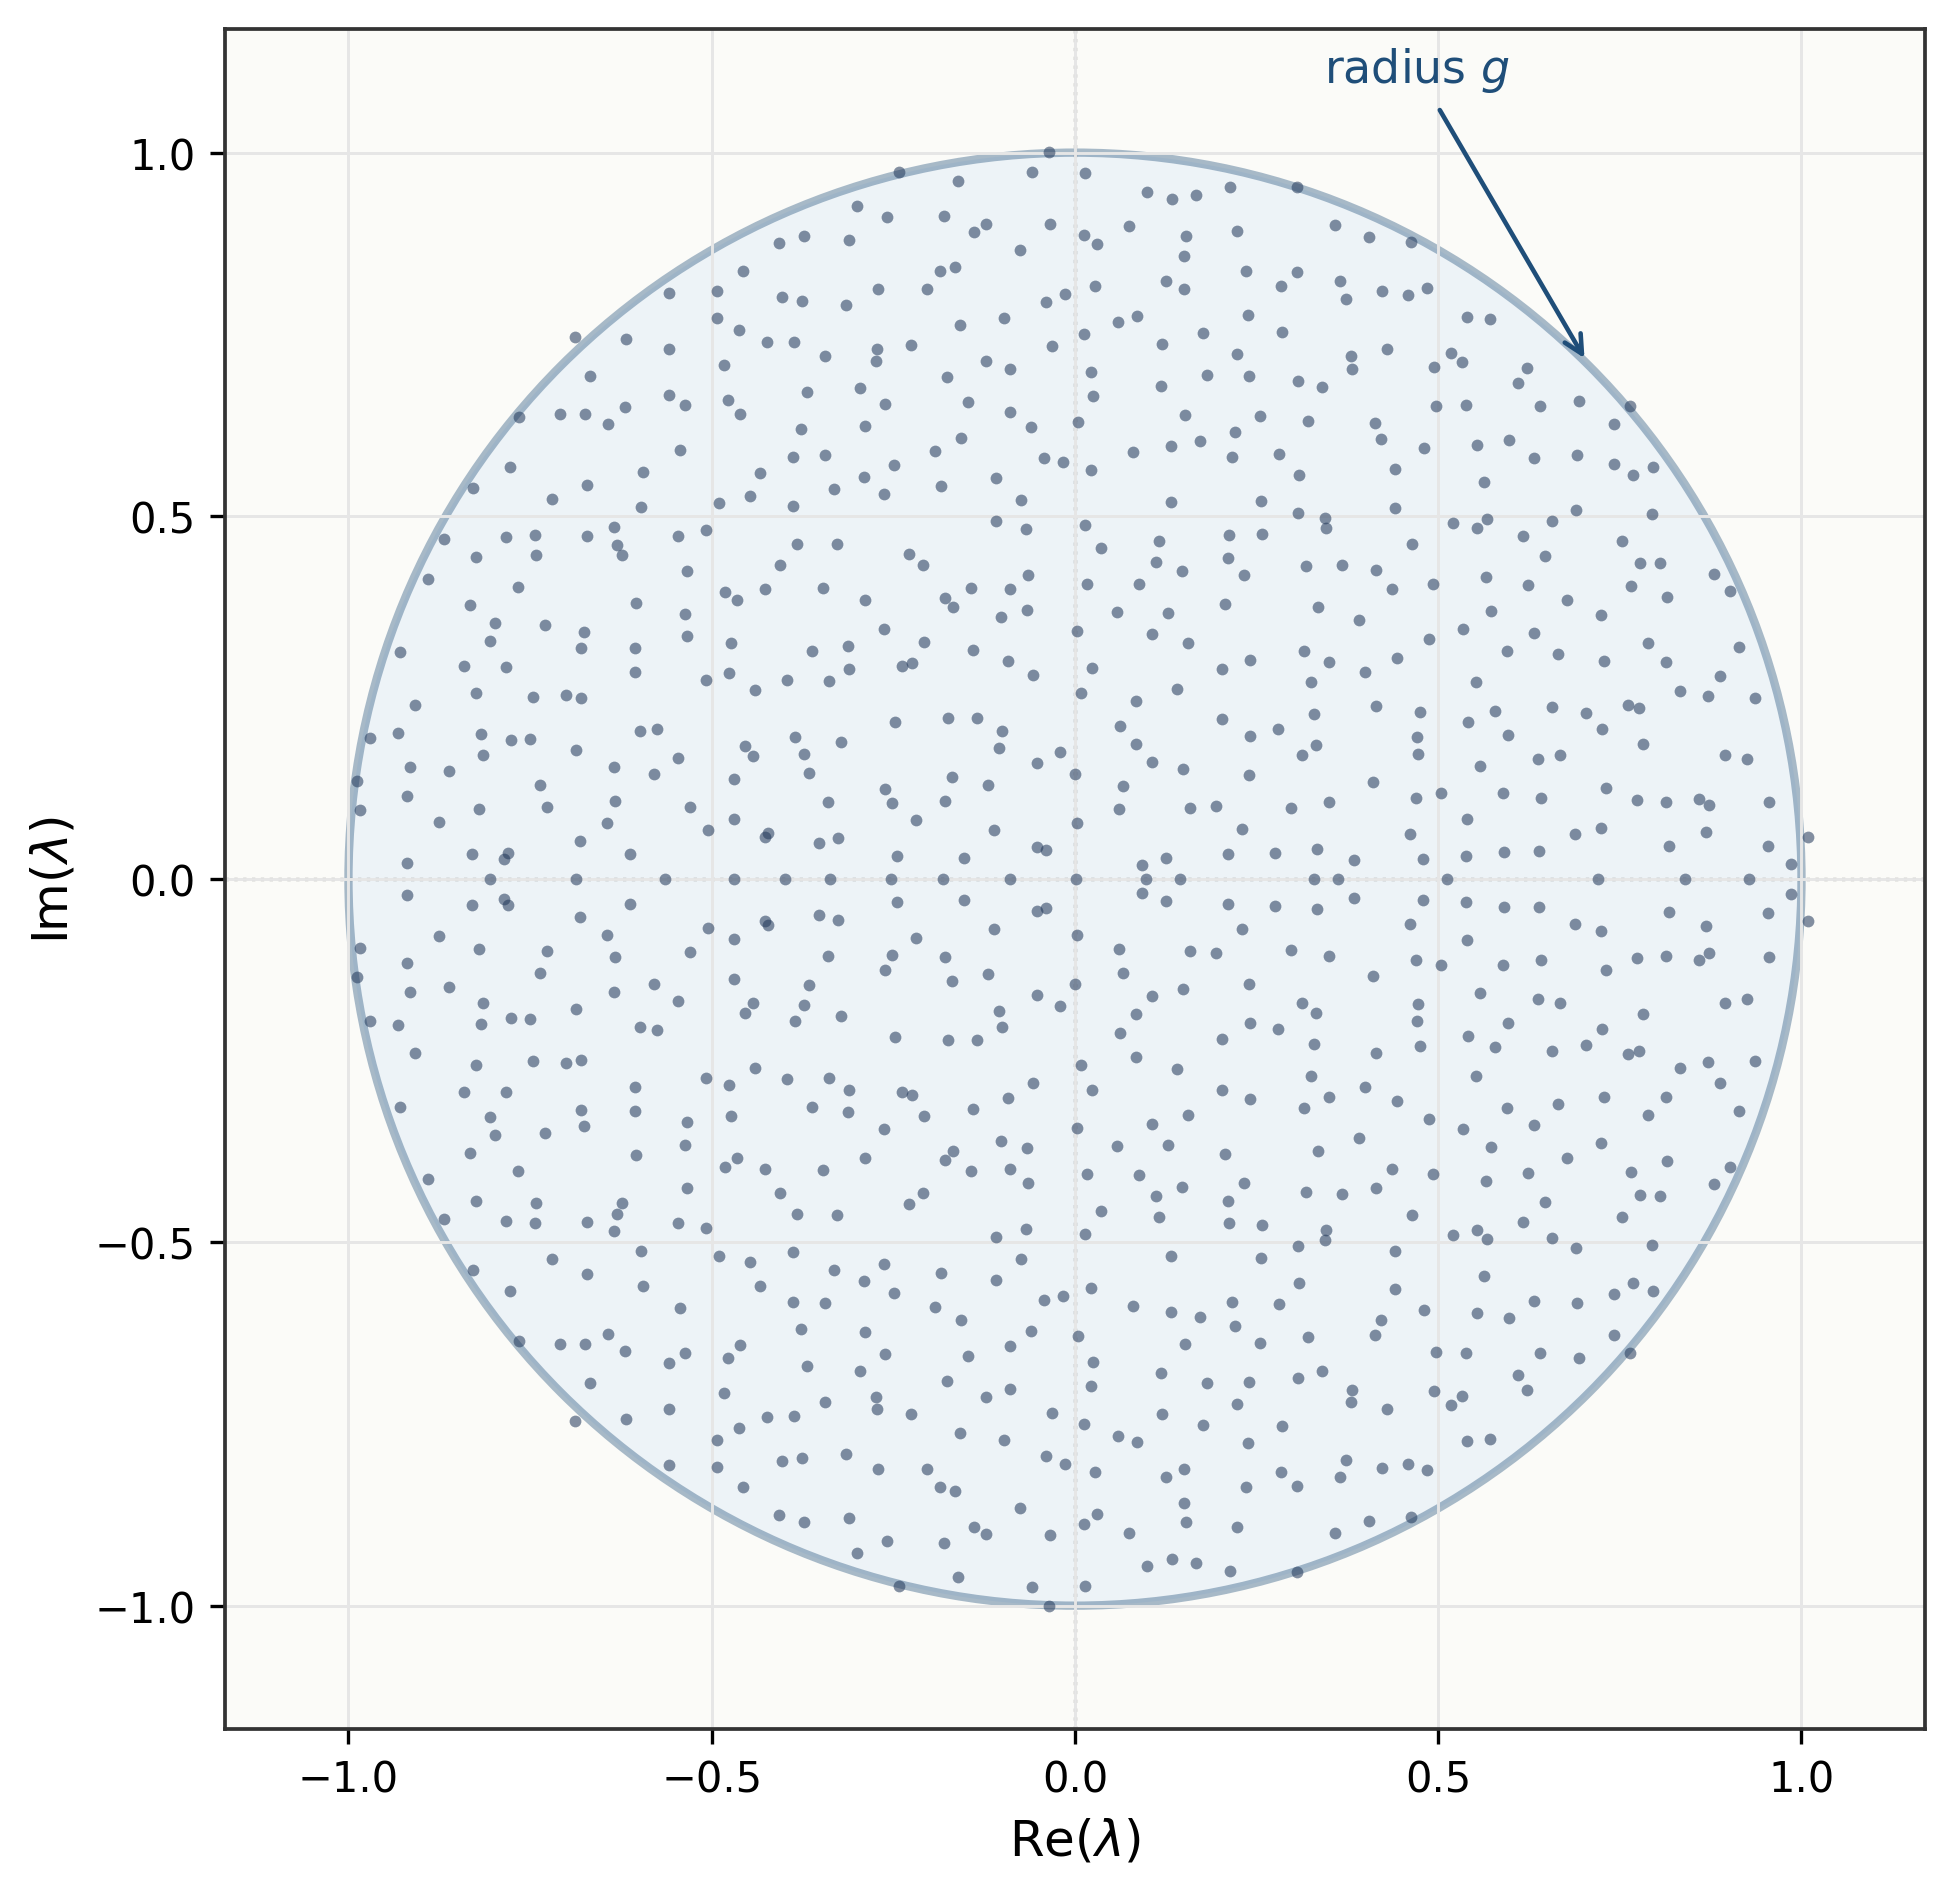
\includegraphics[width=0.45\textwidth]{Girko/girko_circular_law.png}
    \caption{Eigenvalues of a random weight matrix $W \in \mathbb{R}^{n \times n}$, $W_{ij} \sim \mathcal{N}(0, \frac{g}{n^2})$, $n=900$ uniformly distributed on the disk \(D_g\) of radius \(g\) in accordance with Girko's circular law.}
    \label{fig:girko}
\end{figure}
\FloatBarrier

The "gain" parameter, $g$, thus controls spectral radius $\rho(W) \approx g$ which in turn determines strength of recurrent feedback. 
%----------------------------------------------------------------------------------------
%	THEORETICAL SECTION
%----------------------------------------------------------------------------------------
\section{Theoretical Analysis}
\subsection{Fixed-Point Analysis TODO: FIX TITLE}
Suppose that we randomly initialize the interneural weights for a neural network as above. Formally, encode this is $W \in \mathbb{R}^{n \times n}$ with $W_{ij} \sim \mathcal{N}(0, \frac{g^2}{n})$ where $n$ is the number of neurons in our network. To simplify analysis, a neuron is also initialized with a random self-recurrent connection. Througout our analysis in this paper, we shall use $\tanh$ as our activation function for its nonlinear, smooth, zero-centered, and bounded behavior. 

First, we briefly analyze the undriven behavior of the fixed-weight system, that is, we analyze

\[
\tau \dot{\mathbf{x}}  = -\mathbf{x} +  \tanh(W {\mathbf x}).
\]
Here, we apply hyperbolic tangent elementwise; that is,
\[\tau \dot{x_i} = -x_i + \tanh(\sum_{j}W_{ij}x_j)\]
Linearizing around the origin yields the Jacobian
\[
J(0) = \frac{1}{\tau}(- \text{Id} + W). 
\]

Each eigenvalue $\lambda$ of $W$ corresponds to eigenvalue 
\[
\mu = \frac{\lambda - 1}{\tau}
\]
of $J(0)$. By Girko's circular law, the eigenvalues of $W$ approximately fill the disk
$|\lambda| \leq g$, so the Jacobian eigenvalues fill the shifted disk
$|\tau\mu + 1| \leq g$.  The rightmost point of this disk lies at
\[
\Re(\mu)_{max} \approx \frac{g-1}{\mu}
\]
Consequentially, we expect that the origin is stable for $g < 1$ and unstable for $ g > 1$, with $g=1$ some Jacobian eigenvalues cross the imaginary axis and the origin becomes unstable; perturbations
can be amplified by recurrent feedback. Thus, $g=1$ here serves as a bifurcation point. 

\subsection{Stability and Existence Arguments}
\hl{ ADI} 
\subsection{Averaging Analysis and Slow-manifold dynamics}
A key assumption in our analysis is the seperation of time scales in neural activity and Oja-type learning. Assume that
\[\tau \ll \frac{1}{\eta}\]
so that the neural activity evolves on a much faster time scale than that of the weights. In our simulations, we use $\eta = 0.01$ ($1/\eta = 100$) and $\tau = 1$. \\

On the fast activity timescale, $W$ is approximately constant. Section~$4.2$ then predicts that $\mathbf{x}(t)$ settles into a unique periodic orbit, $\mathbf{x}(t; W)$, of frequency $\omega$ determined by the current weight matrix $W$. Now, we shall use averaging theory to characterize dynamics on the slow manifold. Averaging over one drive period $T_d = 2 \pi / \omega$ yields the slow-manifold dynamics

\[
\dot{W_{ij}} \approx \eta[C_{ij}(W) - C_{ii}(W)W_{ij}] - \lambda W_{ij}
\]
where
\[
C(W) = \frac{1}{T_{d}} \int_{0}^{T_d}\mathbf{x}(t; W)\mathbf{x}(t;W)^T \, dt
\]
is the time-averaged correlation matrix of the neural activity. Setting $\dot{W}_{ij} = 0$ yields the fixed point condition
\[
W_{ij}^* = \frac{\eta C_{ij}(W^*)}{\eta C_{ii}(W^*) + \lambda}. 
\]
For $\mathbf{x}(t) = \mathbf{x}$, that is constant neural activity, the above equation reduces to 
\[
W_{ij}^* = \frac{x_ix_j}{\eta{x_i}^2 + \lambda} = u_ix_j, \qquad u_i = \frac{\eta x_i}{\eta x_i^2 + \lambda},
\]
so
$W = ux^T.$
Thus, we have that a fixed point in this neural-weight augmented system corresponds to a rank-one weight matrix. \\

For sinusoidal drive drive at frequency $\omega$, we have that every \hl{explain before why frequency is omega} neuron responds at the same frequency $x_i(t) \approx r_i\sin(\omega t + \theta_i)$. We then have that the time-averaged correlation matrix is 
\[
C_{ij}(W) \approx \frac{1}{2}r_ir_j\cos(\theta_i - \theta_j)
\]
Letting $a_i \coloneq r_i\cos(\theta_i)$ and $b_i \coloneq r_i \sin (\theta_i)$, we have
\[
C(W) \approx \frac{1}{2}(aa^T + bb^T)
\]
and is thus of rank at most $2$. Now, when in the saturated regime of weight dynamics, $x_i \to \pm 1$ is a fixed point \hl{CHARACTERIZE STABILITY OF THIS FIXEDP POINT AND FORMALLY JUSTIFY}. Thus, $C_{ii} = x_i^2 \to 1$ as our activity saturates. We thus have the following
\[
W^{*} \approx \frac{\eta}{\eta + \lambda}C(W^*)
\]
and since $C(W)$ is positive semi-definite,
\[
\rho(C(W)) \le \max_i{\|\lambda_i\|} \le \operatorname{tr}(C) \approx n
\]
under saturation, and so 
\[
\rho(W^*) \le \frac{\eta}{\eta + \lambda}\operatorname{tr(C)} \approx \frac{n \eta}{\eta + \lambda}.
\]

So, we have approximated an upper bound on the spectral radius of the saturated system. \\

\hl{Adi can you check this} If we additionally assume that under saturation, the phases of the neural activities approximately align, then $\cos(\theta_i - \theta_j) \approx 1$ and so 
\[
C(W^*) \approx \frac{1}{2}(aa^T + bb^T) \approx \frac{1}{2}rr^T
\]
collapses to a rank 1 matrix. We obtain an explicit estimate of spectral radius
\[
\rho(W^*) \approx \frac{\eta}{\eta + 2\lambda}\|r\|^2
\]
under this approximation. Since each neuron saturates to $r_i^2 \approx x_i^2 = 1$, we obtain
\[
\rho(W^*) \approx \frac{n\eta}{\eta+ 2\lambda}
\]
\\

If we use the parameters from our numerical simulations, specifically $n=50$, $\eta = 0.01$, and $\lambda = 0.001$, the first approximation yields
\[
\rho(W^*) \le 45.5
\]
and the second approximation yields
\[\rho(W^*) \approx 41.7.\]

\subsection{Effective Random-Matrix Gain}
Although the nominal spectral radius $\rho(W)$ characterizes the initial random
matrix, the stability of the driven system is governed by $\rho(D(t)W)$, the
spectral radius of the effective recurrent matrix $D(t)W$.  Because the entries of
$D(t)W$ are $d_i(t) W_{ij}$, and $W_{ij}$ has variance $g^2/n$, conditional on
$D(t)$ we have that

\begin{equation}
    \mathrm{Var}\bigl((D(t)W)_{ij}\bigr) = \frac{g^2\,d_i(t)^2}{n}.
\end{equation}

Applying Girko's law to $D(t)W$ motivates what we denote
\textit{effective gain}

\begin{equation}
    g_{\mathrm{eff}}(t) \approx \frac{\|W(t)\|_F}{\sqrt{n}}\sqrt{\frac{1}{n}\sum_{i=1}^n d_i(t)^2}.
    \label{eq:geff}
\end{equation}

 Where we approximate
 \[
 \mathbb{E}[\|W(t)\|^2_F] = \sum_{i,j}\mathbb{E}[W_{ij}^2(t)] = n^2 \cdot \frac{g^2}{n} = ng^2
 \]
 under the assumption that $W_{ij}$ remain approximately i.i.d of mean $0$ and variance $g^2/n$. Because $W$ is not stationary, this approximation becomes weaker as the system evolves;  however, numerical simulations demonstrate the effectiveness of $g_{eff}$ in approximation $\rho(D(t)W)$ in the short-term. When neurons are
unsaturated ($d_i \approx 1$), $g_{\mathrm{eff}} \approx g$. Under strong periodic
drive, neurons saturate ($|h_i| \to \infty$, $d_i \to 0$), pulling $g_{\mathrm{eff}}$
below $g$ regardless of spectral radius of $W$. 

%----------------------------------------------------------------------------------------
%	NUMERICAL SECTION
%----------------------------------------------------------------------------------------
\section{Numerical Simulations}
\hl{May need to fix titles for the graphs}
This section provides a series of numerical results which test a variety of hypotheses and properties of the system with Oja-type plasticity. All simulations use networks of $n = 50$ neurons with $\tau = 1$, $\eta = 0.01$,
$\lambda = 0.001$, sinusoidal drive amplitude $A = 1$, and frequency $\omega = 1$
unless otherwise specified.  Random phase offsets $\phi_i \sim \mathrm{Uniform}(0,2\pi)$
are drawn independently for each neuron so that the population-averaged input
correlation matrix is not trivially rank-one by construction.  Results are averaged
over 5 random seeds with error bars showing one standard deviation.

\subsection{Oja Learning Does Not Self-Organize to the Edge of Chaos}

A motivation for studying recurrent neural networks with Oja-type plasticity was to study the hypothesis that perhaps such a learning rule may reorganize weights to the edge of chaos, allowing for optimal signal reconstruction. To test this hypothesis, we sweep initial spectral radii $g_0 \in \{0.3, 0.5, 0.7, 1.0, 1.5, 2.0, 2.5\}$ and run the full coupled system

\begin{align}
    \tau \dot{x}_i &= -x_i + \tanh\!\Bigl(\textstyle\sum_j W_{ij}x_j + A\sin(\omega t + \phi_i)\Bigr), \nonumber\\
    \dot{W}_{ij} &= \eta\,x_i(x_j - x_i W_{ij}) - \lambda W_{ij},
\end{align}

\hl{FIX THE TITLE IN THIS CHART AND MAKE IT BIGGER}

for $T = 400$ time units under both sinusoidal drive ($A=1$) and autonomous dynamics ($A=0$).

\begin{figure}[H]
    \centering
    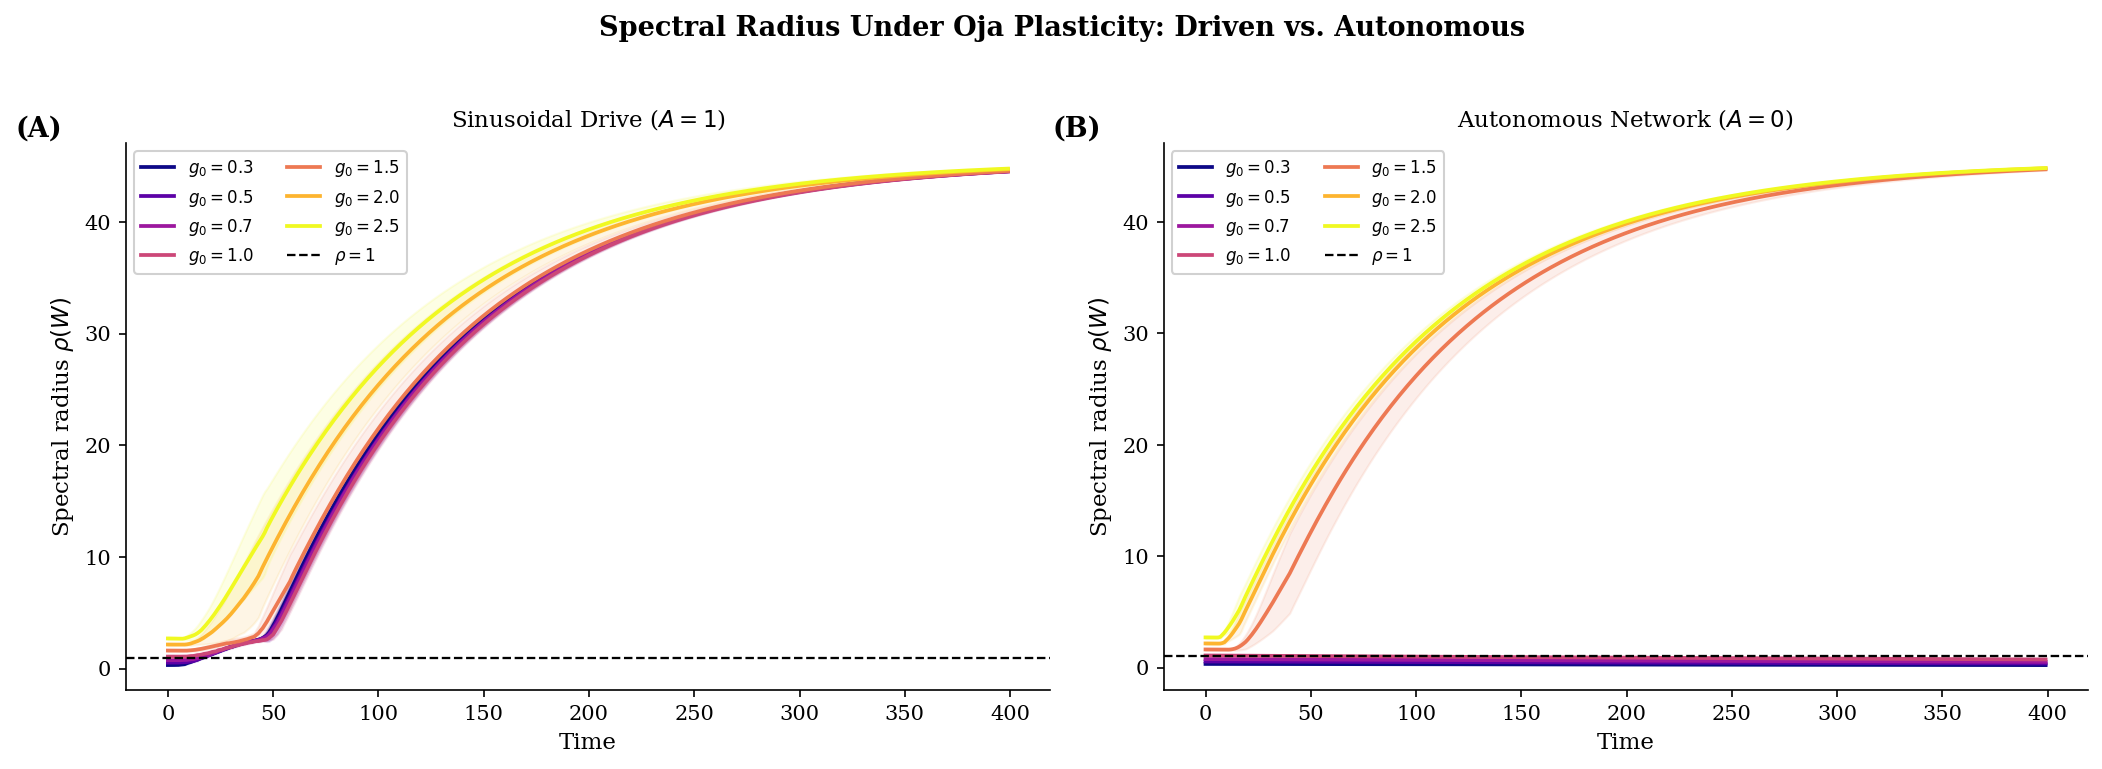
\includegraphics[width=0.75\textwidth]{oja_chaos/spectral_radius_trajectories.png}
    \caption{Spectral radius $\rho(W(t))$ over time for all initial conditions $g_0$
    under sinusoidal drive (left) and autonomous dynamics (right).}
    \label{fig:rho_traj}
\end{figure}
\hl{Fix image formatting and text captions}
Under sinusoidal drive ($A=1$), the spectral radius of the blows up for all initial conditions ($\rho(W) \to 45$ for every initial $g_0$), with all
trajectories converging within $T \approx 150$ time units (Figure~\ref{fig:rho_traj}).
The drive erases all memory of the initial condition. The autonomous system ($A=0$), on the other hand, exhibits a bifurcation at $g_0 = 1$.

These results suggest that addition of periodic input
erases this bifurcation, removing the stable branch near $\rho(W) = 1$.  The
mechanism reflects the analysis in Section~4.3 where the sinusoidal driver creates a low-rank structure which mutually amplifies the spectral radius until the upper bound imposed by the bounded non-linear activation function is reached. The spectral radius in the numerical simulations approaches $45.455$. This suggests that the $x_i$ indeed saturate to approximately $\pm 1$. The assumption that neural phases align however seems to be weaker, which is likely explained by the non-linear distortion of assumed sinusoidal neural activity. 



\subsection{Edge-of-Chaos Optimality for Signal Reconstruction}

While we find that Oja learning does not maintain the network near the edge of chaos, we expect that the
initial spectral radius $g$ still determines the quality of signal reconstruction
during the early learning transient, before the dimension of the weight matrix collapse. For each $g_0$, we run the driven Oja system
for $T = 80$ time units, ideally long enough for activity transients to decay (since $\tau=1$)
but short enough that Oja has not yet fully saturated the network
($\rho(W) \approx 10$--$20$). We then fit a linear readout to reconstruct
$y(t) = \sin(\omega t)$ from the activity history $X \in \mathbb{R}^{T/dt \times n}$, the idea being that the set of sinusoidal waves serves as a basis for periodic functions:

\begin{equation}
    \mathbf{c}^* = \arg\min_{\mathbf{c}}\,\|X\mathbf{c} - \mathbf{y}\|^2,
    \qquad
    R^2 = 1 - \frac{\|X\mathbf{c}^* - \mathbf{y}\|^2}{\mathrm{Var}(\mathbf{y})}.
\end{equation}

\begin{figure}[H]
    \centering
    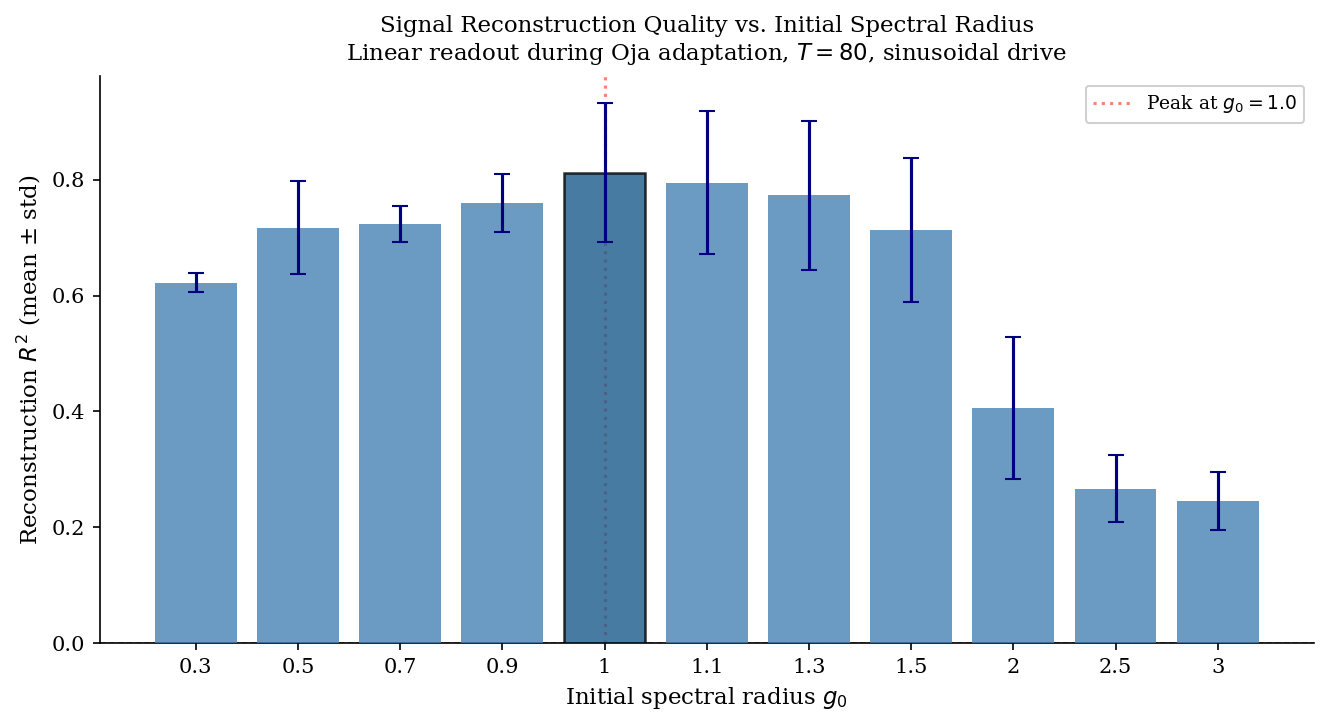
\includegraphics[width=0.7\textwidth]{oja_chaos/r2_vs_g.png}
    \caption{Signal reconstruction $R^2$ as a function of initial spectral radius $g_0$.}
    \label{fig:r2_vs_g}
\end{figure}

$R^2$ peaks at $g_0 \approx 0.9$--$1.0$, reaching $R^2_{\max} \approx 0.81 \pm 0.06$,
and falls to $R^2 \approx 0.22$ at $g_0 = 3.0$ (Figure~\ref{fig:r2_vs_g}).  These results suggest that networks
initialized at the edge of chaos produce the richest activity during the learning
transient, allowing more accurate signal reconstruction before Oja-learning saturates the system, in turn degrading
signal diversity. This is consistent with the theoretical reservoir computing model, where proximity to the edge of chaos maximizes the effective useful dimensionality
of the network's response \hl{Adi, can you check if this is justified}. 


\subsection{Frozen Random Reservoir Outperforms Oja-Learned Weights}

To isolate the degradation of the quality in  signal reconstruction from Oja-type learning, we compare this with a frozen random reservoir.
For each $g_0$, we keep the weights fixed (i.e., $\eta, \lambda = 0$) and fit a ridge-regression
readout with regularization $\alpha = 10^{-3}$. Ridge-regression was used here to account for potential unstable least-squares regression in the high-dimensional, noisy data. 

\begin{equation}
    \mathbf{c}^* = (X^TX + \alpha I)^{-1}X^T \mathbf{y}.
\end{equation}
where $\mathbf{y} = \sin(\omega \mathbf{t})$. 
\begin{figure}[H]
    \centering
    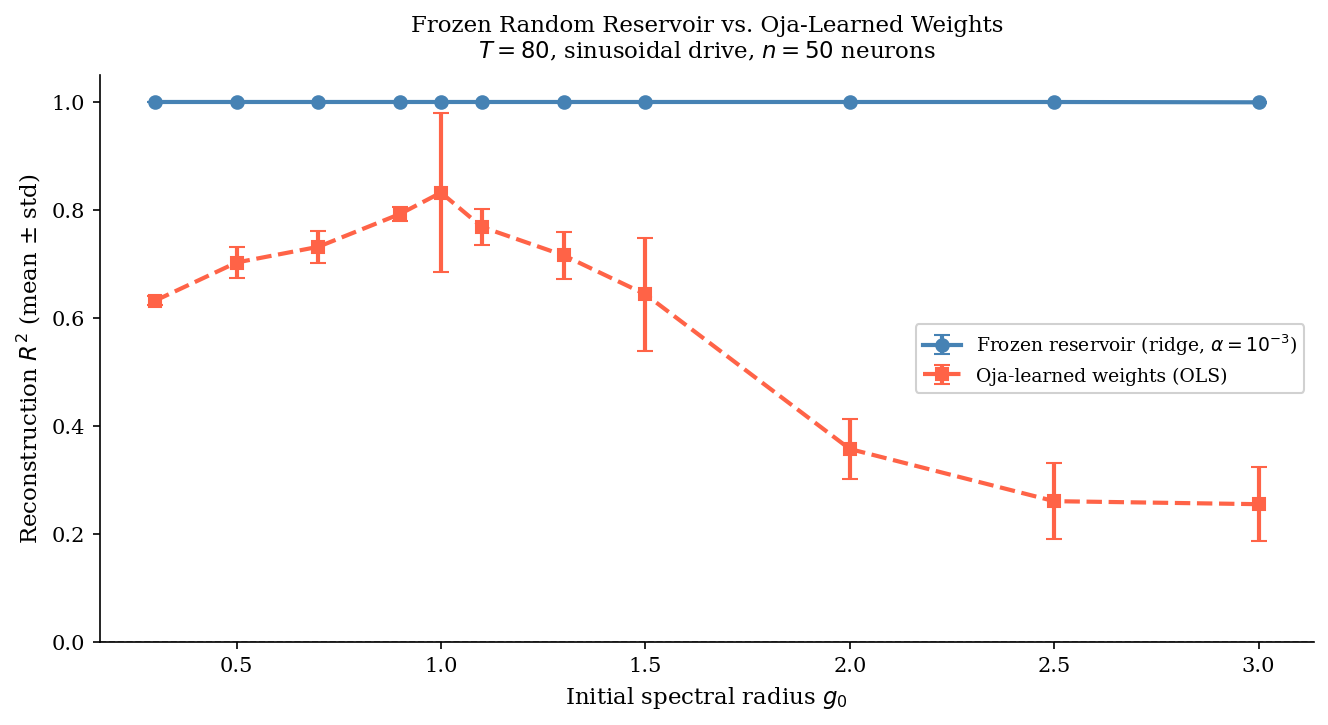
\includegraphics[width=0.7\textwidth]{network_analysis/r2_baseline_vs_oja.png}
    \caption{Comparison of signal reconstruction $R^2$ for Oja-learned weights
    (orange) versus a frozen random reservoir with ridge regression (blue).}
    \label{fig:r2_comparison}
\end{figure}

The frozen reservoir achieves $R^2 \approx 1.0$ for every $g_0$
(Figure~\ref{fig:r2_comparison}). Even this is not a trivial result: the neural network transforms the input sine waves into neural responses with varying amplitude, phases, and nonlinear distortions. On the other hand, Oja-type learning consistently performs worse, driving $\rho(W) \to 45$,
saturating the bounded hyperbolic tangent nonlinearity and degrading the activity diversity in neural activity that allows for high signal reconstruction quality. The frozen network, though, retains useful diversity in neural activity for all $g_0$. \\

\subsection{Input Structure Drives Rank Collapse}

The separation of time scales analysis (Section~4.3) predicts that rank collapse is tied to the
rank of $C(W)$, not to the learning rule itself.  We test this by replacing the
sinusoidal drive with three alternatives:

\begin{itemize}
    \item \emph{Quasi-periodic:} $\frac{A}{\sqrt{3}}\sum_{k=1}^3 \sin(\omega_k t + \phi_i)$,
          with $\omega_1 = 1$, $\omega_2 = \varphi$ (golden ratio), $\omega_3 = \sqrt{2}$
          (chosen to be mutually incommensurate frequencies).
    \item \emph{White noise:} $\xi_i(t) \sim \mathcal{N}(0, A^2/2)$ drawn independently
          for each neuron at each timestep
    \item \emph{Zero drive:} $A = 0$ (autonomous network).
\end{itemize}
The paremeters of each system here were chosen to match $A\sin(\omega t)$ in power, which we use as a proxy for input strength, in order to isolate the effects of the temporal structure on the system (with obvious exception of the autonomous network). 

\begin{figure}[H]
    \centering
    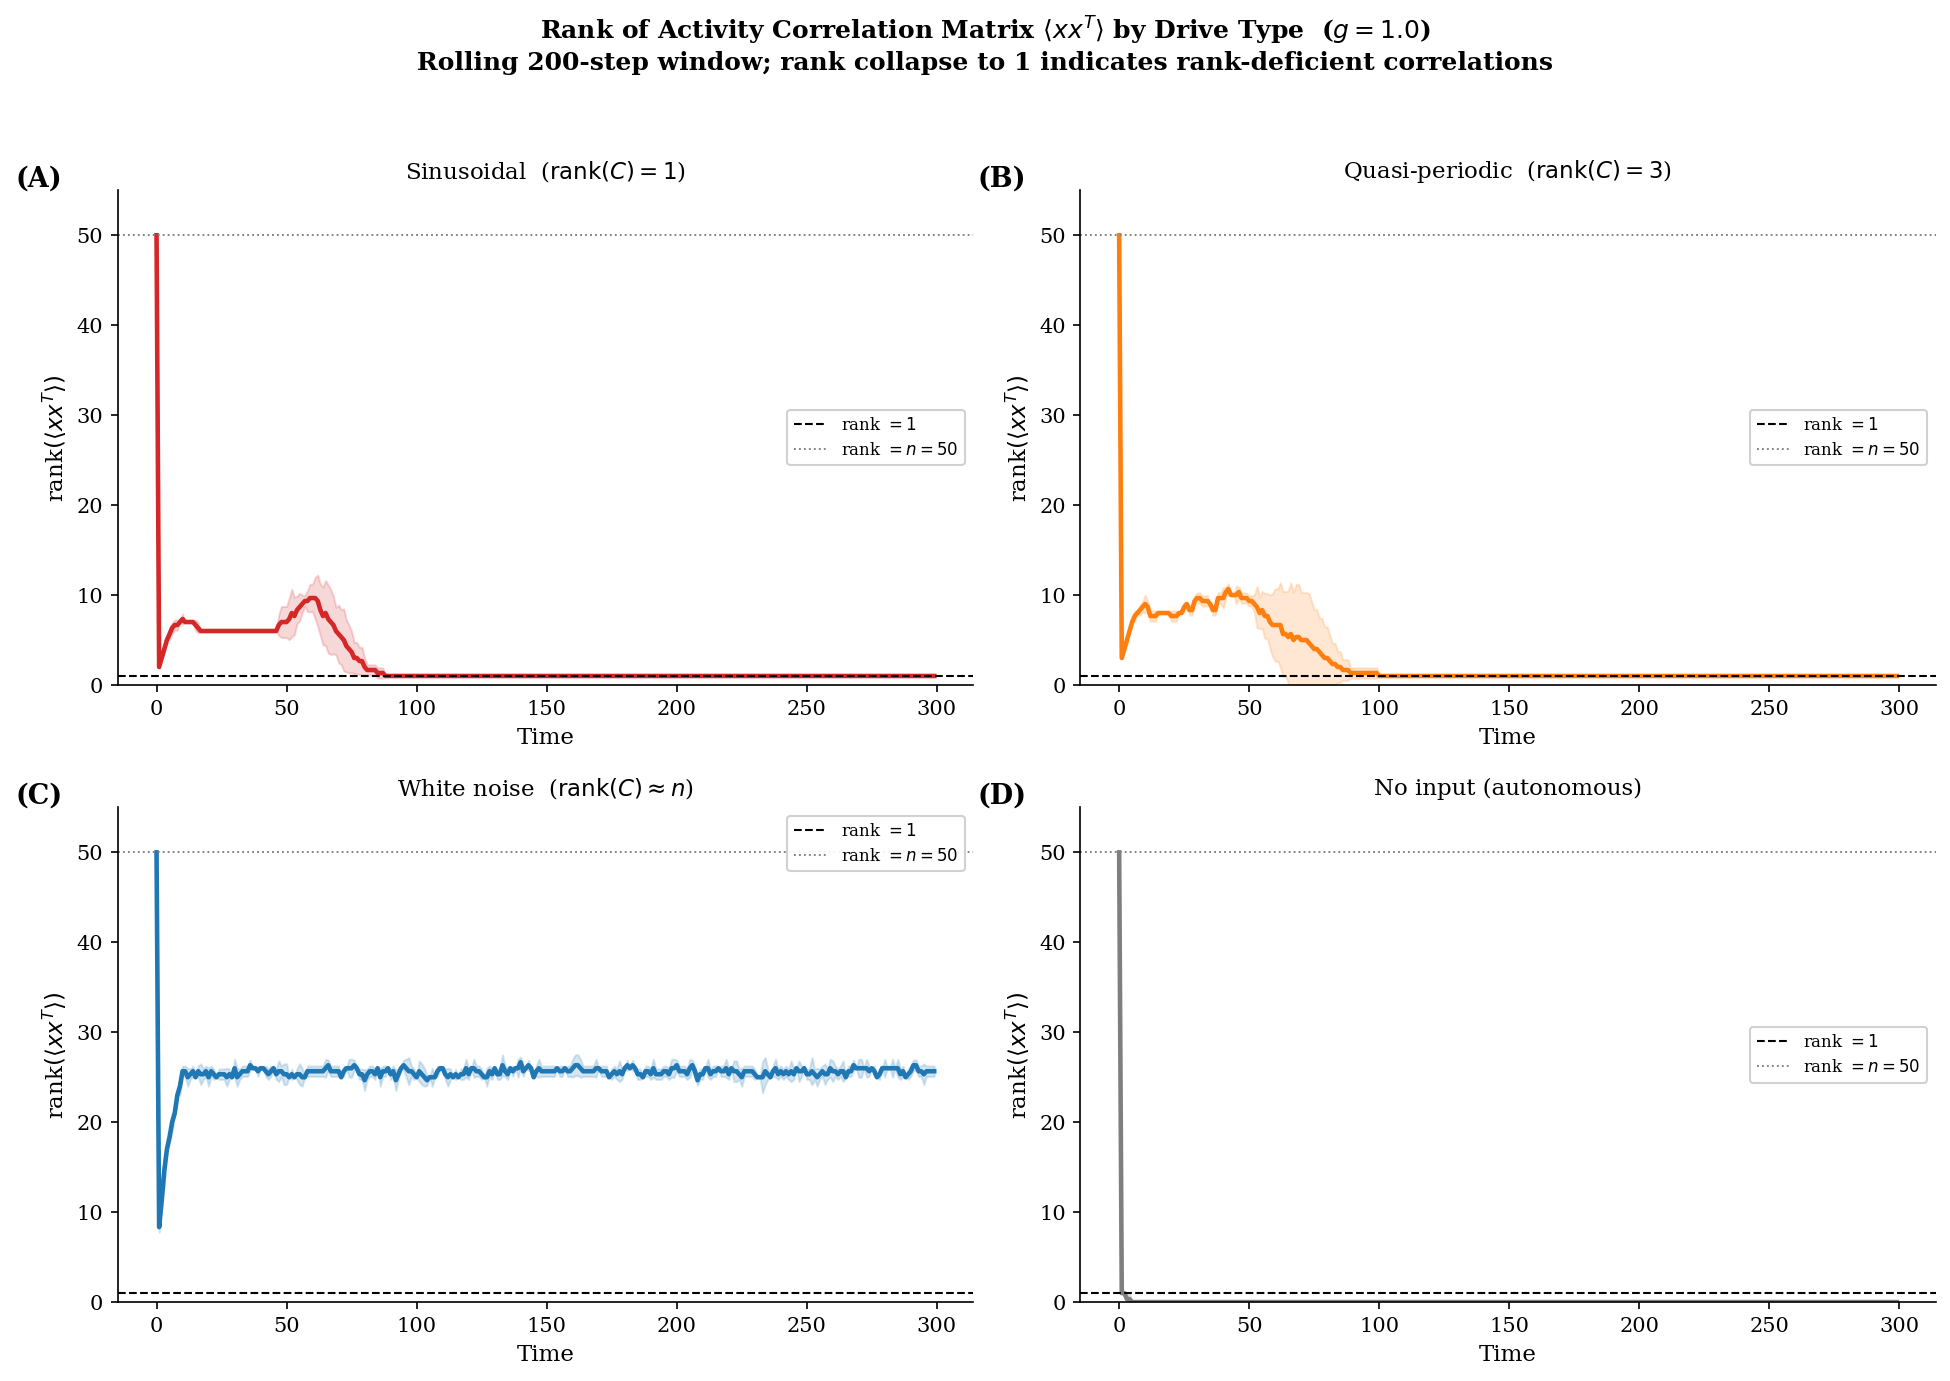
\includegraphics[width=0.85\textwidth]{signal_comparison/correlation_rank_by_drive.png}
    \caption{Rank of the rolling activity correlation matrix $\hat{C}$ over time for
    all four drive types at $g = 1.0$, using a 2000-step (100 time unit) rolling window.
    Sinusoidal (A) and quasi-periodic (B) drives collapse the rank to 1; white noise (C)
    preserves the full rank $n = 50$; the autonomous network (D) silences to rank~0.}
    \label{fig:rank_collapse}
\end{figure}

With a 2000-step (100 time unit) rolling window, the results reveal a clear pattern
across all four drive types (Figure~\ref{fig:rank_collapse}).  Sinusoidal drive
collapses $\mathrm{rank}(\hat{C}) \to 1$ within $T \approx 100$ time units (panel A).
Quasi-periodic drive with three mutually incommensurate frequencies produces nearly
identical collapse, reaching $\mathrm{rank}(\hat{C}) \approx 1$ by $T \approx 150$
time units (panel B).  Both structured drives push $\rho(W) \to 43$ regardless of
initial spectral radius.

White noise preserves full-rank correlations: $\mathrm{rank}(\hat{C}) \to n = 50$ in
steady state (panel C).  The isotropic structure of white noise gives
$C \approx \sigma^2 I$, so $W^* \approx (\eta\sigma^2/\lambda) I$ is full-rank with
bounded spectral radius.  In the autonomous case ($A = 0$, panel D), the network
silences at $g = 1$: without external drive, the stable fixed point at the origin
dominates, yielding $\mathrm{rank}(\hat{C}) \to 0$.

These results confirm that rank collapse is driven by the temporal structure of the
input, not by Oja learning alone.  The quasi-periodic result is particularly striking:
three mutually incommensurate frequencies are still insufficient to prevent collapse.
The crucial distinction is not the number of active spectral modes but whether the
input correlation matrix $C$ has low rank---any finite set of periodic components
produces a finite-rank $C$ that Oja then amplifies to drive $\rho(W) \to 45$.


\subsection{Effective Gain Is Self-Regulated by Saturation}

In this section, we seek to validate the heuristic effective gain in two complementary experiments. 

In the first experiment, we track $g_{\mathrm{eff}}(t)$ during Oja
learning alongside $\rho(W(t))$ for sinusoidal and white noise drives.  Under sinusoidal drive, we find that $\rho(W)$ approaches approximately $43$ but every neuron saturates ($|h_i| \to \infty$), so
$d_i = \operatorname{sech}^2(h_i) \to 0$ and $g_{\mathrm{eff}} \to 0$.  Here, the system is in a maximally saturated state where the linearized perturbation dynamics
 are always stable despite the exploding nominal spectral radius.

In our second experiment, we freeze the weights ($\eta, \lambda = 0$) and scan
$g \in [0.1, 3.0]$ with sinusoidal drive, averaging $g_{\mathrm{eff}}$ and $\rho(D(t)W)$
over the steady-state window $t \in [210, 300]$. \hl{Quickly revise the first experiment to describe if the same thing is done}

\begin{figure}[H]
    \centering
    
\includegraphics[width=0.7\textwidth]{geff/geff_static_scan.png}
    \caption{Time-averaged effective gain $g_{\mathrm{eff}}$ (blue) and directly calculated spectral radius
    $\rho(D(t)W)$ (orange) versus nominal $g$ for frozen weights under sinusoidal
    drive. The dotted diagonal shows the no-saturation baseline $g_{\mathrm{eff}} = g$.}
    \label{fig:geff_scan}
\end{figure}

Here we see that heuristic tracks the "effective" spectral radius of the system, $\rho(D(t)W(t))$, within 5\% across all tested $g$
(Figure~\ref{fig:geff_scan}).  The $g_{\mathrm{eff}} = 1$ crossing occurs at
$g \approx 1.5$: sinusoidal drive saturates neurons enough to reduce the effective
gain by approximately 33\%, shifting the effective stability boundary substantially
above the Girko prediction $g = 1$. \hl{How is $g$ caluclated here?} \hl{Revise the first section slightly to clarify that weights here were frozen to isolate the DW dynamics }


\subsection{Critical Slowing Down at the Phase Transition}

Independent evidence for the $g = 1$ phase transition comes from the autonomous
discrete map $h_{t+1} = Wf(h_t)$.  The largest Lyapunov exponent (LLE) $\lambda_1$
is estimated via a 300-step warmup followed by 800-step single-vector power iteration
on the tangent map $J_t = W\operatorname{diag}(\operatorname{sech}^2(h_t))$.  For
$\lambda_1 < 0$ the system is stable with relaxation time
$\tau_{\mathrm{relax}} = -1/\lambda_1$; for $\lambda_1 > 0$ the map is chaotic.
In the linear regime a small perturbation $\delta h(0)$ is predicted to grow as
$\|\delta h(t)\| \approx \varepsilon\,e^{\lambda_1 t}$.

\begin{figure}[H]
    \centering
    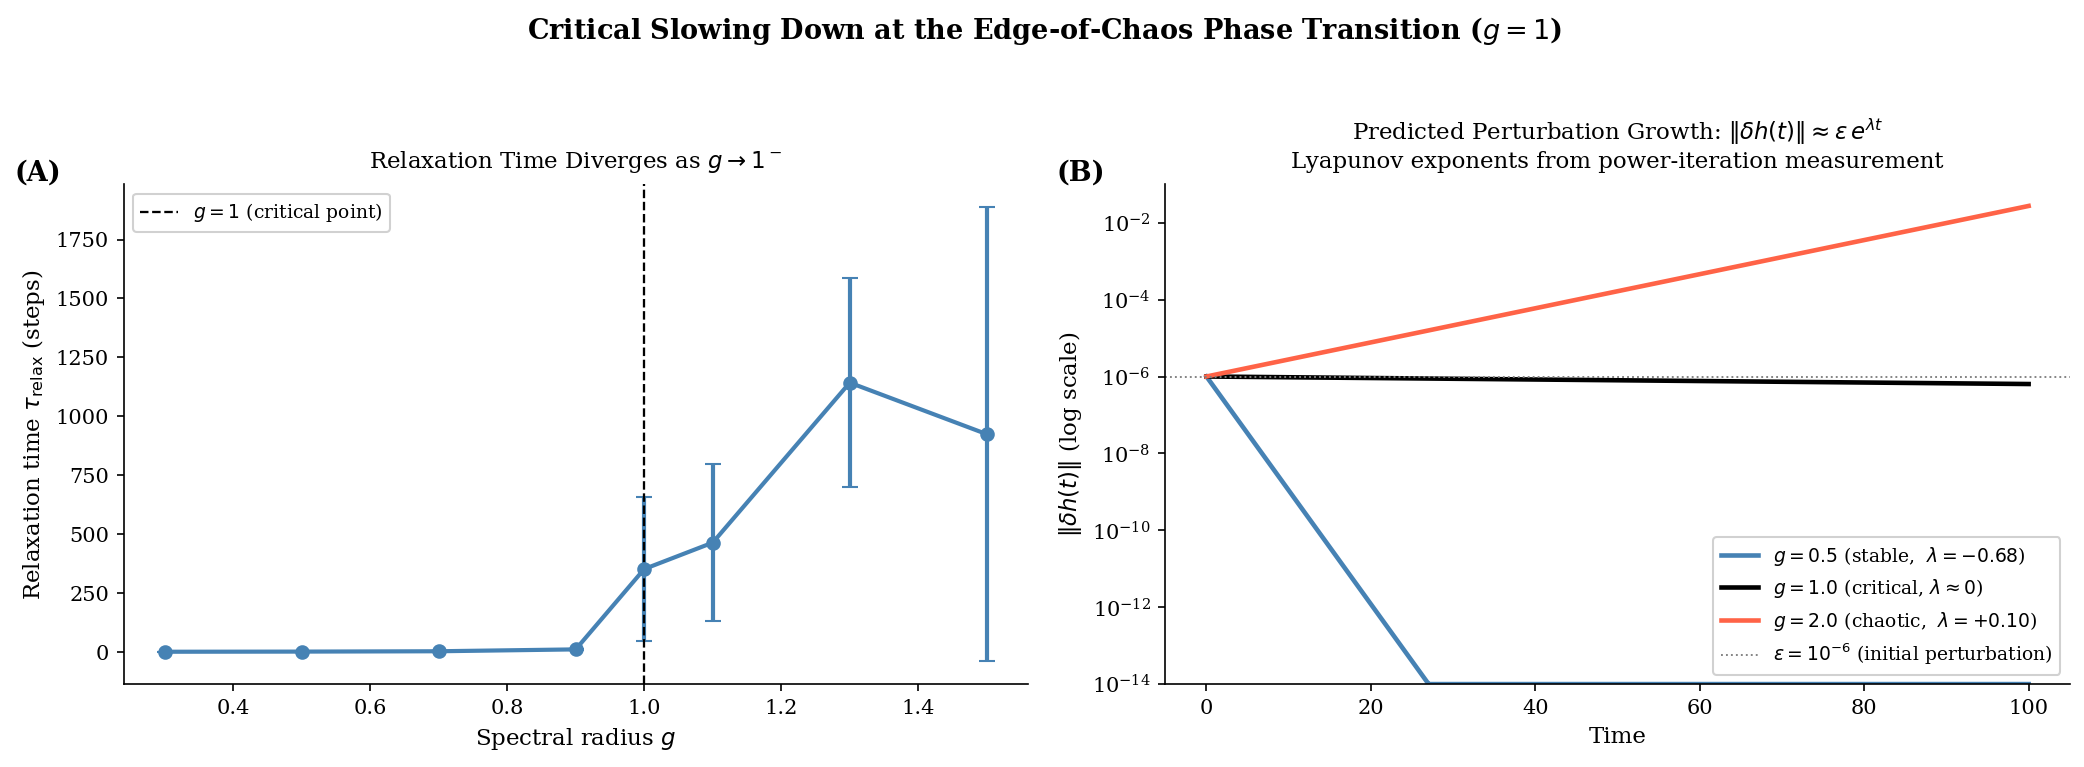
\includegraphics[width=0.85\textwidth]{network_analysis/critical_slowing_down.png}
    \caption{Left: relaxation time $\tau_{\mathrm{relax}} = -1/\lambda_1$ versus $g$
    for the autonomous discrete map; $\tau_{\mathrm{relax}}$ diverges as $g \to 1^-$.
    Right: predicted perturbation growth $\|\delta h(t)\| = \varepsilon\,e^{\lambda_1 t}$
    using the power-iteration LLE values, illustrating the stable ($g = 0.5$), critical
    ($g = 1.0$), and chaotic ($g = 2.0$) regimes.}
    \label{fig:csd}
\end{figure}

\begin{table}[h]
    \centering
    \caption{Largest Lyapunov exponent and relaxation time for selected $g$ values
    ($n = 50$, autonomous discrete map, mean over 5 seeds).}
    \label{tab:lle}
    \begin{tabular}{lrr}
    \toprule
    $g$ & $\lambda_1$ (nats/step) & $\tau_{\mathrm{relax}}$ (steps) \\
    \midrule
    $0.30$ & $-1.20$ & $0.8$ \\
    $0.70$ & $-0.35$ & $2.9$ \\
    $0.90$ & $-0.10$ & $10.8$ \\
    $1.00$ & $-0.005$ & $\approx 350$ \\
    $2.00$ & $+0.10$  & (chaotic) \\
    \bottomrule
    \end{tabular}
\end{table}

Table~\ref{tab:lle} and Figure~\ref{fig:csd} show that $\tau_{\mathrm{relax}}$
diverges as $g \to 1^-$, which is the defining signature of a continuous (second-order)
phase transition \cite{guckenheimer1983nonlinear}.  At $g = 1$ the network has no
preferred timescale for returning to equilibrium: small disturbances persist
arbitrarily long.  This critical slowing down provides a physically clean signature
of the edge-of-chaos transition that is observable independently of the sign of the
LLE.

A note on finite-size effects: Sompolinsky's mean-field theory \cite{sompolinsky1988chaos}
predicts chaos onset exactly at $g = 1$ in the $n \to \infty$ limit.  For $n = 50$,
the discrete map remains stable up to $g \approx 1.5$ (LLE $\approx -0.009$); positive
LLE first appears near $g \approx 2.0$ (Table~\ref{tab:lle}).  The $\tau_{\mathrm{relax}}$
divergence near $g = 1$ is nonetheless clearly visible and confirms the qualitative
picture even at finite $n$.



\section{Conclusions}

%----------------------------------------------------------------------------------------
%	REFERENCES 
%----------------------------------------------------------------------------------------
\clearpage
\nocite{*}
\bibliographystyle{plain}
\bibliography{references}


\end{document}